\chapter{Hardware setup}\label{ch:hardware}
A personal computer has been used to connect with the camera and the robot. The camera was placed inside the robot cell, above the blocks, such that the images were taken from above. This cenital point of allows to efficiently determine the positions and orientations of the blocks. 

The phisical connections to the computer were made through: 
\begin{itemize}
	\item Ethernet to the robot  
	\item USB to the camera 
\end{itemize}

\begin{figure}[hb]
\centering
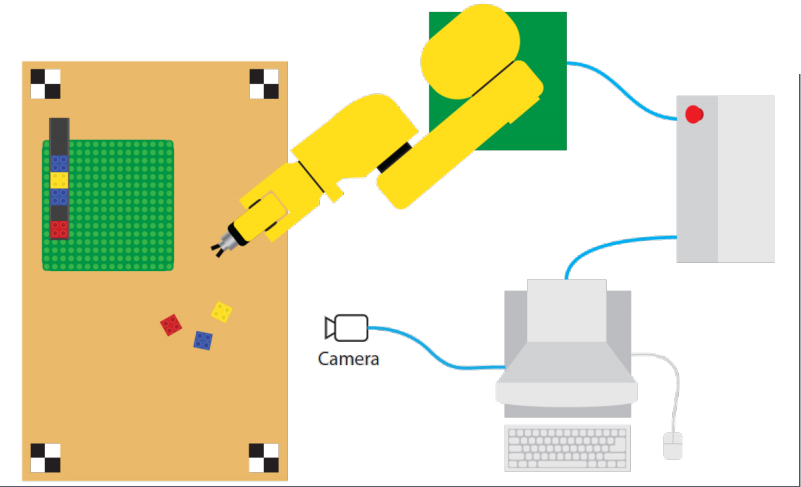
\includegraphics[width=4in]{figures/robotCellDesign.png}
\caption[robot Cell Design]
{An illustration of the hardware setup}
\end{figure}

In order to connect between the different components described above, a local network was set up in which both the computer and the Adept cobra controller were given an static IP. This computer runs the ADEPT Desktop program that was used to send the program code to the robot. This configuration allowed us to communicate with the robot and send Matlab commands to it. MATLAB also includes a camera toolbox to work with it. 
